%%%%%%%%%%%%%%%%%%%%%%%%%%%%%%%%%%%%%%%%%%%%%%%%%%%%%%%%%%%%%%%%%%%%%%%%%%%%%
%
%  System        : 
%  Module        : 
%  Object Name   : $RCSfile$
%  Revision      : $Revision$
%  Date          : $Date$
%  Author        : $Author$
%  Created By    : Robert Heller
%  Created       : Sat Mar 4 08:39:57 2023
%  Last Modified : <230304.1211>
%
%  Description 
%
%  Notes
%
%  History
% 
%%%%%%%%%%%%%%%%%%%%%%%%%%%%%%%%%%%%%%%%%%%%%%%%%%%%%%%%%%%%%%%%%%%%%%%%%%%%%
%
%    Copyright (C) 2023  Robert Heller D/B/A Deepwoods Software
%			51 Locke Hill Road
%			Wendell, MA 01379-9728
%
%    This program is free software; you can redistribute it and/or modify
%    it under the terms of the GNU General Public License as published by
%    the Free Software Foundation; either version 2 of the License, or
%    (at your option) any later version.
%
%    This program is distributed in the hope that it will be useful,
%    but WITHOUT ANY WARRANTY; without even the implied warranty of
%    MERCHANTABILITY or FITNESS FOR A PARTICULAR PURPOSE.  See the
%    GNU General Public License for more details.
%
%    You should have received a copy of the GNU General Public License
%    along with this program; if not, write to the Free Software
%    Foundation, Inc., 675 Mass Ave, Cambridge, MA 02139, USA.
%
% 
%
%%%%%%%%%%%%%%%%%%%%%%%%%%%%%%%%%%%%%%%%%%%%%%%%%%%%%%%%%%%%%%%%%%%%%%%%%%%%%

\documentclass[12pt,twoside]{article}
\usepackage{graphicx}
\usepackage{mathptm}
\usepackage{times}
\usepackage{makeidx}
\usepackage{ifpdf}
\usepackage{footmisc}
\ifpdf
\usepackage[pdftex,
            pagebackref=true,
            colorlinks=true,
            linkcolor=blue,
            unicode
           ]{hyperref}
\else
\usepackage[ps2pdf,
            pagebackref=true,
            colorlinks=true,
            linkcolor=blue,
            unicode
           ]{hyperref}
\usepackage{pspicture}
\fi
\usepackage{url}
\pagestyle{headings}
\makeindex
\emergencystretch=50pt
\setcounter{tocdepth}{3}
\setcounter{secnumdepth}{3}
\title{ESP32 T7S3 MultiFunctionUniversalTurnout Kit Instructions}
\author{Robert Heller \\ The Country Robot \\ Wendell, MA, USA}
\date{\today}
\begin{document}
\maketitle

This is a circuit board that supports a Lily Go T7 S3 (mini32) board to manage
multiple model railroad functions as a LCC\footnote{Layout Command Control --
see NMRA's 9.7.x standards, available on the NMRA website
\url{https://www.nmra.org/lcc}.} node. This board provides the following 
functions:

\begin{itemize}
\item Four turnout motors with point sense.  This board uses one of four 
turnout driver daughter boards:
\begin{enumerate}
\item Stall-motor drivers, suitable for Circuitron Tortoise and similar slow 
motion, stall motor switch machines.
\item Twin-coil drivers, suitable for Atlas or Peco snap action switch 
machines.
\item Single-coil drivers, suitable for Kato snap action switch machines.
\item Servo drivers, suitable for using RC control servos to operate turnouts.
\end{enumerate}
\item Four CT coil occupancy detectors.
\item Four driver circuits, suitable for indicator LEDs, decoupling 
electromagnets, solenoids, relays, etc.
\item Four Schmitt-trigger button inputs.
\item Sixteen signal lamp drivers.
\end{itemize}

\clearpage
\section{Assembly}
\begin{figure}[hbpt]\begin{centering}%
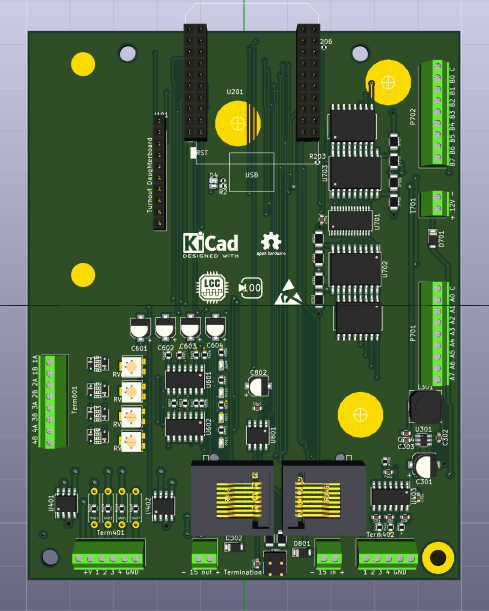
\includegraphics[width=5in]{ESP32-T7S3-MultiFunctionUniversalTurnout.png}
\caption{3D image of the ESP32 T7S3 MultiFunctionUniversalTurnout board}
\end{centering}\end{figure}
\begin{figure}[hbpt]\begin{centering}%
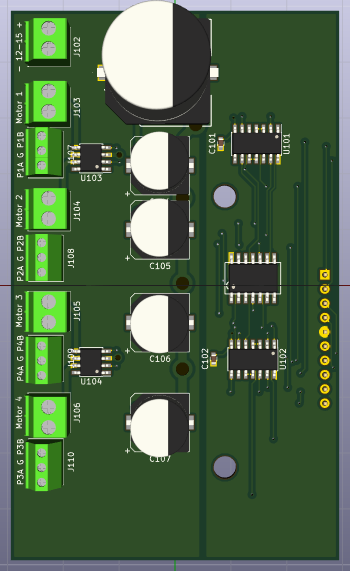
\includegraphics[height=7in]{SC-DaughterBoard.png}
\caption{3D image of the Single Coil Turnout driver daughter board}
\end{centering}\end{figure}
\begin{figure}[hbpt]\begin{centering}%
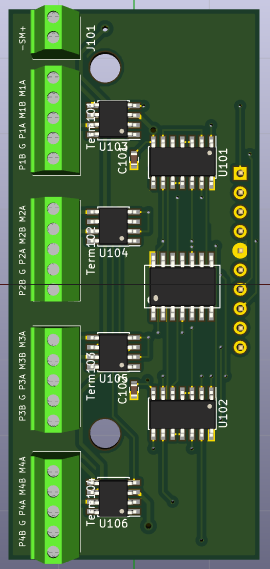
\includegraphics[height=7in]{SM-DaughterBoard.png}
\caption{3D image of the Stall Motor driver daughter board}
\end{centering}\end{figure}
\begin{figure}[hbpt]\begin{centering}%
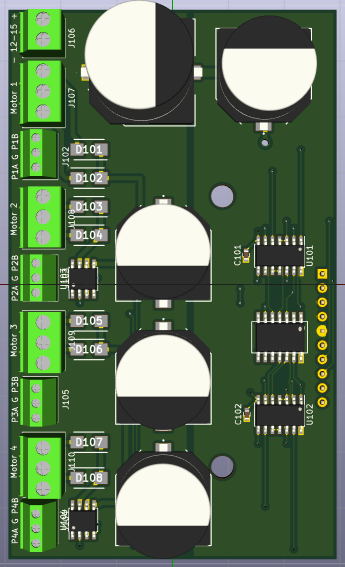
\includegraphics[height=7in]{TC-DaughterBoard.png}
\caption{3D image of the Twin Coil driver daughter board}
\end{centering}\end{figure}
\begin{figure}[hbpt]\begin{centering}%
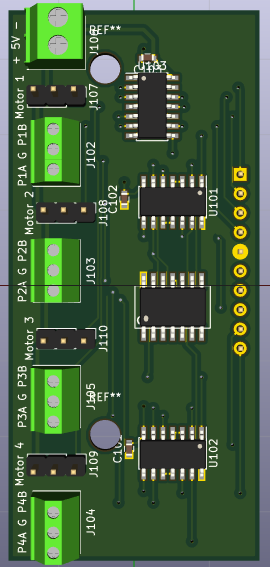
\includegraphics[height=7in]{TS-DaughterBoard.png}
\caption{3D image of the Servo driver daughter board}
\end{centering}\end{figure}

The board has all of the SMD parts factory installed. Only the through-hole
parts are not soldered to the board. These are the RJ45 Jacks, the Termination
Jumper, the turnout daughter board header, the min32 headers, the daughter
board support standoffs, and the terminal blocks. The daughter boards also
have all of the SMD parts factory installed, and just needs their terminal
blocks and board inter-connect headers installed. These are all easy to solder
parts. Make sure the headers and terminal blocks are fully seated and square
to the boards. A simple trick is to solder one pin and then while pressing the
part to the board, reheat that one pin's solder pad and snaping the part to
the board and holding it tight and square to the board as the solder cools.
Important: make sure the wire entry holes in the terminal blocks are facing
the edge of the board! The RJ45 Jacks cannot be installed wrong (they have
orientation pins).  Start with the shortest parts and work up to the tallest.

\clearpage
\section{Downloadables and Software Support}

As shipped, the TTGO-T7S3 has already had the ESP32-S3-MultiFunctionOpenMRNIDF
firmware installed, but if you want to rebuild the code (possibly with
customizations) the code is on GitHub in my ESP32-LCC repo:
\url{https://github.com/RobertPHeller/ESP32-LCC}, in the
ESP32-S3-MultiFunctionOpenMRNIDFOpenMRNIDF sub-folder. You will need the
Espressif's IoT Development Framework, version 4.2 or later, available from
\url{https://github.com/espressif/esp-idf}. The
ESP32-S3-MultiFunctionOpenMRNIDFOpenMRNIDF also uses Mike Dunston's OpenMRNIDF
module. Also available in the 
ESP32-T7S3-MultiFunctionUniversalTurnout/KitBooklet sub-folder are pdfs of the 
circuit diagrams.


\subsection{Building and installing the software}

Once you have installed Espressif's IoT Development Framework and cloned the 
ESP32-LCC repo, you can build the software by cd'ing to the 
ESP32-S3-MultiFunctionOpenMRNIDF and in bash running these commands:

\begin{verbatim}
. path-to-Espressifs-IDF/export.sh
idf.py set-target esp32s3
idf.py menuconfig
idf.py build
\end{verbatim}

Things to check in the menuconfig (under ``Advanced Configuration''):

\begin{itemize}
\item{Using TTGO-T7S3} Turn this option on.
\item{Using the servo turnout daughter board} If you are using the TS (turnout 
servo) daughter board, turn this on.  If using any of the other turnout 
daughter boards turn this off.
\end{itemize}

You can then use the idf.py's flash command to flash the TTGO-T7S3.

\subsection{Program Description}

The program consists of a main sketch file, and several support files and
``components'' (libraries).

\subsection{Program Startup notes}

While most of the common node configuration is accessable using the available
CDI configuruation tools (JMRI's PanelPro program or MRR SYS OpenLCB program),
some of the node's configuration is in separate non-volitle (flash) memory.
This includes the node's ID number and some boot options. As installed the
node ID is initialized to 05:01:01:01:22:00. \textbf{You don't really want to
leave this as the node id!} There are two ways to set the node id. One way is
to use a CDI configuruation tool -- the node ID is exposed as a configuration
option. Changing the node id forces a ``factory reset'' on the next boot (and
when you update the configuration with a CDI configuruation tool, the node
will reboot). The other way is during the boot up process. When the node
boots, it waits on the USB serial connection for 10 seconds for any
``keyboard'' response and if it gets a ``keyboard'' response, it enters a
simple command line loop accepting simple commands (mostly single letters). To
use this feature you need to connect a a USB cable between the TTGO-T7S3 and a
computer (eg a PC or Mac) and then connect to the USB Com port with a terminal
program (the Arduino IDE Serial Monitor should work). The commands that the
boot startup command line loop supports are:

\begin{itemize}
\item \textbf{N} Set the node id.  Follow the ``N'' with a 12 digit hex 
number, with optional periods or colons.  Causes a Factory Reset.
\item \textbf{E} Reset events on boot up.
\item \textbf{F} Force a Factory Reset.
\item \textbf{S} WiFi ssid\footnote{Only useful if WiFi is 
enabled.\label{fn:wifi}}. Enter the ssid after the ``S'', leading and trailing 
spaces are stripped off.
\item \textbf{P} WiFi password\footref{fn:wifi}. Enter the password after the 
``P'', leading and trailing spaces are stripped off.
\item \textbf{H} Hostname prefix\footref{fn:wifi}. Enter the hostname prefix 
after the ``H'', leading and trailing spaces are stripped off. The NODE ID in 
hex is appended.  Hostnames are limited to 32 characters.
\item \textbf{W} Enable WiFi\footref{fn:wifi}. Enter ``YES'', ``NO'', 
``ON'', or ``OFF'' after the ``W''.
\item \textbf{T} Test signal lamps\footnote{Each of the signal lamps is 
flashed for 1 second during boot up.}.
\item \textbf{R} Resume.
\end{itemize}

\end{document}
